\chapter{linguaggi liberi deterministici}

\section{PDA e linguaggi deterministici}
\subsection{PDA deterministici}
\dfn{PDA deterministico}{
    Un PDA $N=(\Sigma, Q, \Gamma, \delta, q_0, \bot, F)$ si dice \textbf{deterministico} sse:
    \begin{enumerate}
        \item \(\forall q \in Q, \; \forall z \in \Gamma, \; \big(\forall a \in \Sigma, \; (\delta(q, \epsilon, z) \neq \varnothing \implies \delta(q, a, z) = \varnothing)\big)\)
        \item $\forall q \in Q, \; \forall z \in \Gamma, \; \forall a \in (\Sigma \cup \{\epsilon\}), \; \big(|\delta(q, a, z)| \leq 1\big)$

    \end{enumerate}
}
Ovvero un PDA è libero deterministico sse in ogni configurazione, il PDA ha al massimo una transizione possibile per un dato stato, simbolo di input, e simbolo in cima alla pila e se ha una transizione $\epsilon$ disponibile allora non ha altri tipi di transizioni.

Quindi un PDA:
\begin{itemize}
    \item ha al massimo una transizione
    \item non ha conflitti tra transizioni $\epsilon$ e transizioni che leggono un simbolo
\end{itemize}
\subsection{Definizione di linguaggi liberi deterministici}
\dfn{Linguaggio libero deterministico}{
    Un linguaggio è \textbf{libero deterministico} se è accettato per stato finale da un DPDA
}
\teorema{
    la classe dei linguaggi liberi deterministici è includa propriamente nella classe dei linguaggi liberi :)
}
\esempio{
    \begin{itemize}
        \item Sia $L_1=\{ww^R\mid w\in\{a,b\}^*\}$ è libero, am si può dimostrare che non esiste un DPDA che lo riconosca, infatti con un DPDA non esiste un modo deterministico per riconoscere quando finisce $w$ e inizia $w^R$
        \item $L_2=\{wcw^R\mid w\in\{a,b\}^*\}$ è libero deterministico grazie al segnaposto $c$ è possibile riconoscere quando inizia $w^R$, si ha infatti:
        \begin{tikzpicture}
            % States
            \node[state, initial] (q0) {\(q_0\)};
            \node[state, right of=q0] (q1) {\(q_1\)};
            \node[state, right of=q1] (q2) {\(q_2\)};
            \node[state, accepting, right of=q2] (q3) {\(q_3\)};
            
        
            % Transitions
            \draw (q0) edge[loop above] node[align=center] {\(a, Z \to aZ\) \\ \(b, Z \to bZ\)} (q0);
            \draw (q0) edge[below] node {\(c, Z \to Z\)} (q1);
            \draw (q1) edge[loop above] node[align=center] {\(a, a \to \varepsilon\) \\ \(b, b \to \varepsilon\)} (q1);
            \draw (q1) edge[below] node {\(\varepsilon, Z \to Z\)} (q2);
            \draw (q2) edge[below] node {\(\varepsilon, Z \to \varepsilon\)} (q3);
        
        \end{tikzpicture}        
    \end{itemize}
}
\teorema{
    Se $L$ è regolare, allora $\exists\; DPDA$ $N$ tale che $L=L[N]$ per stato finale
    
  %  \begin{center}
   %     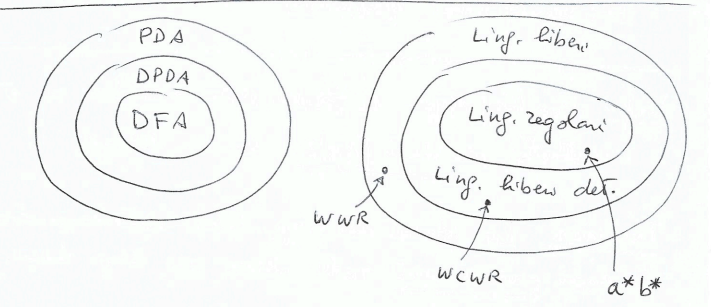
\includegraphics[width=10cm]{gerarchia_automi.png}
    %\end{center}
    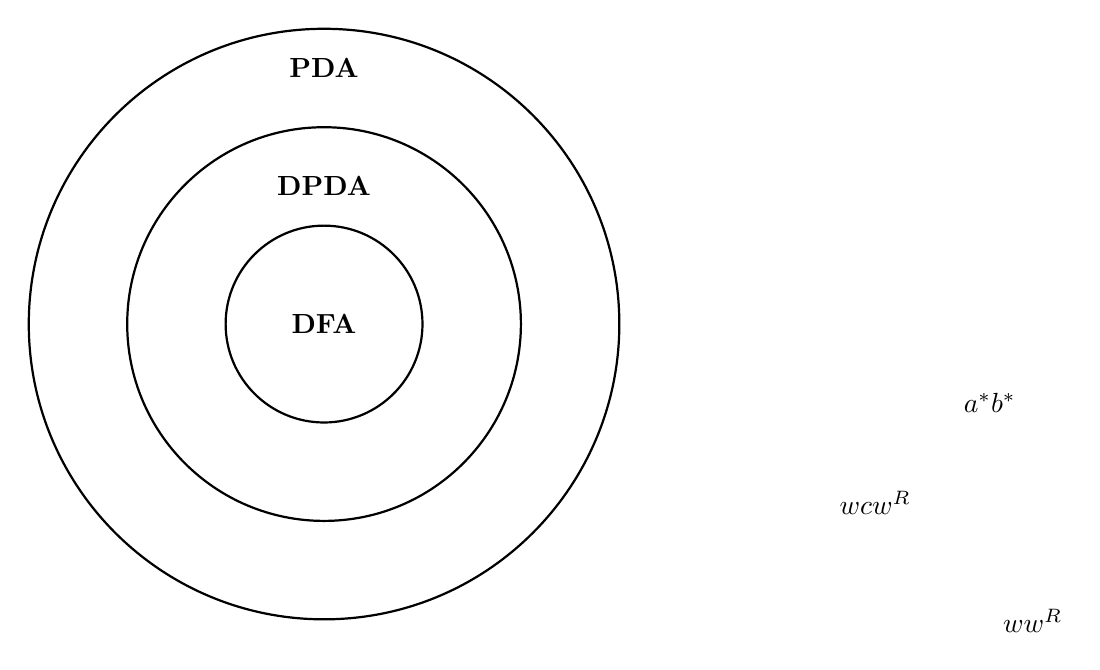
\begin{tikzpicture}
        % Cerchi per gli automi
        \draw[thick] (0, 0) circle (1.25cm) node[pos=0, yshift=0cm] {\textbf{DFA}};
        \draw[thick] (0, 0) circle (2.5cm) node[pos=0, yshift=1.75cm] {\textbf{DPDA}};
        \draw[thick] (0, 0) circle (3.75cm) node[pos=0, yshift=3.25cm] {\textbf{PDA}};
    
        % Cerchi per i linguaggi
        %\draw[thick] (8, 0) circle (1.5cm) node[pos=0, below right, xshift=-1.3cm] {\textbf{Linguaggi regolari}};
        %\draw[thick] (8, 0) circle (3cm) node[pos=0, above right, xshift=-2.1cm] {\textbf{Linguaggi liberi deterministici}};
        %\draw[thick] (8, 0) circle (4.5cm) node[pos=0, above right, xshift=-2.8cm] {\textbf{Linguaggi liberi}};
        
        % Annotazioni linguaggi
        \node[right] at (8, -1) {\(a^*b^*\)};
        \node[below] at (7, -2) {\(wcw^R\)};
        \node[below right] at (8.5, -3.5) {\(ww^R\)};
    \end{tikzpicture}
    
}
\pf{dimostrazione}{
    Se $L$ è regoalre, allora $\exists$ DFA $M$ tale che $L=L[M]$. A partire da $M$, posso costruire un DPDA $N$ si compore come $M$ senza mai manipolare lo stack, allora si che $L=L[N]$ per stato finale 
}
\subsubsection{Prefix propriety}
Si giunge così al seguente fatto:
\clm{}{}{
    Un linguaggio libero deterministico $L$ è riconosciuto da un $DPDA$ per pila vuota sse $L$ gode della "perfix propriety", ovvero 
    \[
        \nexists x,y\in L : x \text{ è prefisso di }y       
    \]
}
Pertanto si ha che:
\begin{itemize}
    \item Se $L$ è non gode della prefix propriety non può essere riconosciuto da un $PDPA$ per pila vuota
    \item Se $L$ è libero deterministico gode della prefix propriety, allora può essere riconosciuto da un $PDPA$ per pila vuota
    \item Se $L$ è libero deterministico, allora $L\$ =\{w\$ \mid w\in L\}$ gode della prefix propriety, infatti $L\$$ può essere riconosciuto da un $PDPA$ per pila vuota.
    
    Dove $\$\notin\Sigma$ ovvero $\$$ non è un simbolo dell'alfabeto di $L$, ma grazie ad esso alla fine di ogni linguaggio regolare vale la prefix propriety
\end{itemize}

\esempio{
    Sia $L_1 = \{a^nb^n\mid n\geq 0\}$ il seguente linguaggio che non gode della prefix propriety, in quanto $\epsilon\in L_1$ e $\epsilon$ è prefisso di $ab$

    \begin{tikzpicture}
        % States
        \node[state, initial, accepting] (q0) {\(q_0\)};
        \node[state, right of=q0] (q1) {\(q_1\)};
        \node[state, right of=q1] (q2) {\(q_2\)};
        \node[state, accepting, right of=q2] (q3) {\(q_3\)};
        
    
        % Transitions
        
        \draw (q0) edge[below] node {$\epsilon, Z/Z$} (q1);
        \draw (q1) edge[loop above] node[align=center] {$a,Z/AZ$} (q1);
        \draw (q1) edge[loop below] node[align=center] {$a,A/AA$} (q1);
        \draw (q1) edge[below] node {$b,A/\epsilon$} (q2);
        \draw (q2) edge[loop above] node[align=center] {$b,A/\epsilon$} (q2);
        \draw (q2) edge[below] node[align=center] {$\epsilon,Z/\epsilon$} (q3);
    
    \end{tikzpicture}
    
    Si ha quindi che il seguente linguaggio è riconosciuto da un DPDA \textit{per stato finale} e non \textit{per pila vuota}. Tuttavia il seguente linguaggio con il $\$\notin\Sigma$ è riconosciuto da un DPDA per \textit{per pila vuota}

    Sia $L_1\$$:


    \begin{tikzpicture}
        % States
        \node[state, initial] (q0) {\(q_0\)};
        \node[state, accepting, below of=q0] (q1) {\(q_1\)};
        \node[state, right of=q0] (q2) {\(q_2\)};
        \node[state, right of=q2] (q3) {\(q_3\)};
        
    
        % Transitions
        
        \draw (q0) edge[below] node {$a, Z/AZ$} (q2);
        \draw (q0) edge[left] node {$\$,Z/\epsilon$} (q1);
        \draw (q3) edge[loop above] node[align=center] {$b,A/\epsilon$} (q3);
        \draw (q3) edge[left] node[align=right] {$\$, Z/\epsilon$} (q1);
        \draw (q2) edge[loop above] node[align=center] {$a,A/AA$} (q2);
        \draw (q2) edge[below] node[align=center] {$b,A/\epsilon$} (q3);
    
    \end{tikzpicture}

    Si verifichi, infatti, come egli venga riconosciuto per pila vuota

}

\esempio{
    Sia $L_3 = \{a^nb^m\mid n\geq m \geq 0\}$ e dato che $\epsilon\in L_3$ tale linguaggio non gode della prefix propriety

    \begin{tikzpicture}
        \node[state, initial, accepting] (q0) {$q_0$};
        \node[state,  accepting, right of=q0] (q1) {$q_1$};
        \node[state,  accepting, right of=q1] (q2) {$q_2$};
        \node[state,  accepting, right of=q2] (q3) {$q_3$};

        \draw (q0) edge[above] node[align=center] {$a,Z/AZ$} (q1);
        \draw (q1) edge[above] node[align=center] {$b,A/\epsilon$} (q2);
        \draw (q2) edge[above] node[align=center] {$\epsilon, Z/\epsilon$} (q3);
        \draw (q2) edge[loop above] node[align=center] {$b,A/\epsilon$} (q2);
        \draw (q1) edge[loop above] node[align=center] {$b,A/AA$} (q1);
        
    \end{tikzpicture}

    e sia $L_3\$$:

    \begin{tikzpicture}
        \node[state, initial] (q0) {$q_0$};
        \node[state,  right of=q0] (q1) {$q_1$};
        \node[state,  right of=q1] (q2) {$q_2$};
        \node[state,  above of=q1] (q3) {$q_3$};
        \node[state,  below of=q1] (q4) {$q_4$};

        \draw (q0) edge[above] node[align=center] {$a,Z/AZ$} (q1);
        \draw (q0) edge[left] node[align=center] {$\$,Z/\epsilon$} (q3);
        \draw (q1) edge[above] node[align=center] {$b,A/\epsilon$} (q2);
        \draw (q1) edge[left] node[align=center] {$\$,A/\epsilon$} (q4);
        \draw (q2) edge[right] node[align=center] {$\$, Z/\epsilon$} (q3);
        \draw (q2) edge[right] node[align=center] {$\$, A/\epsilon$} (q4);

        \draw (q2) edge[loop right] node[align=center] {$b,A/\epsilon$} (q2);
        \draw (q1) edge[loop above] node[align=center] {$b,A/AA$} (q1);
        \draw (q4) edge[loop left] node[align=center] {$\epsilon,X/\epsilon$} (q4);

        
    \end{tikzpicture}


}

\subsubsection{non ambiguità dei linguaggi liberi deterministici}
\mprop{}{
    Se $L$ è libero deterministico, ovvero riconosciuto da un $DPDA$ per \textit{stato finale}, allora $L$ è generabile da una \textbf{grammatica libera non ambigua}.
    
    Si ha quindi che i \red{linguaggi liberi deterministici non sono ambigui}
}


%! errori e non capisco il motivo puercos zios
\subsubsection{Proprietà dei linguaggi liberi deterministici}

I lunguaggi liberi deterministici presentano le seguenti proprietà:
\mprop{chiusura solo per complementazione}{
    Sia $L$ un linguaggio libero deterministico, allora questo è chiuso per complementazione, ovvero:
    \[
        (\exists \; \text{DPDA} \; N \; : \; L = L(N)) \implies (\exists \; \text{DPDA} \; N' \; : \; \overline{L} = L(N')) \quad \text{dove} \quad \overline{L} = \Sigma^* \setminus L

    \]
}
\dimostrazione{
    Bisogna rendere totale la $\delta$ di $N$, eventualmente aggiungendo stati non finali, e poi $N'$ si ottiene da questo $N$ "aumentato", semplicemente scambiando \red{finali e non finali} 
}

\mprop{
    Non chiusura per intersezione
}{
    Un linguaggio libero deterministico non è chiuso per intersezione
}
\esempio{
    $L_1 =\{a^nb^nc^m\mid n,m\geq 0\}$ è libero deterministico\\
    $L_2 =\{a^mb^nc^n\mid n,m\geq 0\}$ è libero deterministico\\
    ma\\
    $L_1\cap L_2 =\{a^nb^nc^n\mid n\geq 0\}$ non è libero!

}

\mprop{
    non chiusura per unione
}{
    Un linguaggio libero deterministico non è chiuso per unione
}
\dimostrazione{
    Assumiamo per assurdo che un linguaggio libero deterministico sia chiuso per unione, allora:
    \[
        L_1\cap L_2 = \overline{\overline{L_1}\cup \overline{L_2}}    
    \]

    Per questo fatto e la proprosizione precedente si è verificato un assurdo
}

\subsection{Analizzatori sintattici: parser}
\begin{tikzpicture}[node distance=2cm]

        % Nodes
        \node (grammar) [startstop] {Grammatica Libera};
        \node (algorithm) [process, right of=grammar, xshift=4cm] {Algoritmo di \\ Costruzione (YACC)};
        \node (parser) [startstop, right of=algorithm, xshift=4cm] {Parser};
        \node (tokens) [startstop, below of=grammar, yshift=-2.5cm] {Lista di Token};
        \node (parser2) [process, right of=tokens, xshift=4cm] {Parser};
        \node (tree) [startstop, right of=parser2, xshift=4cm] {Albero di Derivazione};
        \node (additional) [below of=parser] {fondamentalmente un \\$DPDA$ con output};
        
        % Arrows
        \draw [arrow] (grammar) -- (algorithm);
        \draw [arrow] (algorithm) -- (parser);
        \draw [arrow] (tokens) -- (parser2);
        \draw [arrow] (parser2) -- (tree);
        \draw [wavearrow] (additional) -- (parser)
        
        % Additional text
        
        
        
        
\end{tikzpicture}

I parser possono essere:
\begin{itemize}
    \item \textbf{nondeterministici}: se, durante la ricerca di una derivazione, si scopre che una scelta è improduttiva e non porta a riconoscere l'input, \red{il parser torna indietro} (\textit{backtracking}), disfa parte della derivazione appena costruita e scegli un'altra produzione, \red{tornando a leggere parte dell'input}
    \item \textbf{deterministici}: leggono l'input una sola volta ed \red{ogni loro decisione è definitiva}
\end{itemize}

entrambi cercano di sfruttare informazioni dall'input per guidare la ricerca della derivazione

\subsubsection{introduzione al top-down parsing}
\dfn{}{
    Data $G=(NT,T,S,R)$ lebera, costruiamo il $PDA\;M=(T,\{q\}, T\cup NT, \delta, q, S, \varnothing)$, che riconosce per pila vuota, dove $\delta:Q\times(\Sigma\cup\{\epsilon\})\times\Gamma→Q\times\Gamma^*$ è definita:
    \begin{itemize}
        \item \textbf{espandi}: $(q,\beta)\in \delta(q,\epsilon, A)$ se $A\to\beta\in R$ 
        \item \textbf{consuma}: $\forall a\in T((q,\epsilon)\in \delta(q,a, a))$ 
    \end{itemize} 
    Tale che $L(G)=P[M]$ (riconoscimento per pila vuota)
}

Quindi, grazie alla prima regola se il simbolo in cima alla pila è un non terminale $A$, l'automa può espanderlo sostituendolo con la produzione $\beta$, come descritto nelle regole $R$ della grammatica, mentre secondo la regola di consumazione si ha che se il simbolo sulla cima della pila e il simbolo corrente della stringa in input sono entrambi a, allora l'automa può eliminare quel simbolo dalla pila e procedere nella lettura dell'input.

\esempio{
    Sia $G$ la seguente grammatica:
    \[
        \begin{array}{l}
            S\to aSb\mid \epsilon
        \end{array}    
    \]

    Si ha che $S\implies aSb \implies aaSbb \implies aabb$

    \begin{center}
       \begin{tikzpicture}
        \node[state] (q) {$q_0$};
        \draw (q) edge[loop right] node[align=center] {$b,b/\epsilon$} (q);
        \draw (q) edge[loop above] node[align=center] {$a,a/\epsilon$} (q);
        \draw (q) edge[loop left] node[align=center] {$\epsilon,S/\epsilon$} (q);
        \draw (q) edge[loop below] node[align=center] {$\epsilon,S/aSb$} (q);
    \end{tikzpicture} 
    \end{center}

    Si osservi che il seguente automa che riconosce il linguaggio della grammatica $S$ non è un PDPA

    Nella maggior parte delle configurazioni standard di un Pushdown Automaton (PDA) utilizzato per il parsing top-down, la pila viene inizializzata con il simbolo iniziale della grammatica, nel nostro caso, quindi, la serie di passaggi che porteranno a riconoscere il linguaggio sarà:
    \[
        \begin{array}{l}
            (q,aabb,S) \vdash (q,aabb,aSb)\\
            \vdash (q,abb,Sb)\vdash (q,abb,aSbb)\\
            \vdash  (q,bb,Sbb)\vdash (q,bb,bb)\\
            \vdash (q,b,b)\vdash (q,\epsilon,\epsilon)
        \end{array}
    \]
    che costruisce il seguente albero di derivazione 
    \begin{center}
        \begin{tikzpicture}
            \Tree [.S 
                        a
                        [.S
                            a
                            [.S
                                $\epsilon$
                            ]
                            b
                        ]
                        b
                ]
        \end{tikzpicture}
    \end{center} 

    Si ha, quindi:
    \begin{itemize}
        \item derivazione canonica a sx (leftmost)
        \item costruzione dell'albero dall'alto in basso
    \end{itemize}

    %TODO triangolo
}

Tuttavia in questo esempio è facile verificare che il parser è nondeterministico, infatti l'automa è un $PDA$, tuttavia questo nondeterminismo può essere risolto \red{scegliendo la produzione in baso al simbolo di lettura nell'input} (\textbf{look-ahead}), ad esempio:
\begin{itemize}
    \item se leggo $a$, espando $S\to aSb$
    \item se leggo $b$, espando $S\to \epsilon$
\end{itemize}

\begin{center}
  \begin{tabular}{rrr}
    \textbf{input} & \textbf{stack}&\textbf{azione}\\
    $\underline{a}abb\$$&$S$&leggo $a$ e espando in $aSb$ \\
    & $\underline{a}Sb$&consumo\\
    $\underline{a}bb\$$&$Sb$&leggo $a$ e espando in $aSb$\\
    &$\underline{a}Sbb$&conumo\\
    $\underline{b}b\$$ & $Sbb$&leggo $b$ e espando in $\epsilon$\\
    &$\underline{b}b$&consumo\\
    $b\$$&$b$&leggo $b$ e espando in $\epsilon$ \\
    $\$$ & $\epsilon$& fin
\end{tabular}  
\end{center}

\nt{
    Non tutte le grammatiche sono adatte per il top down-parser
}
\esempio{
    Sia $G$ la segnuete grammatica:
    \[
        S\to Sb\mid a        
    \]
    e $L(G)=ab^*$ (linguaggio regolare semplice)

    L'automa che riconosce il linguaggio è:
    \begin{center}
        \begin{tikzpicture}
         \node[state] (q) {$q$};
         \draw (q) edge[loop right] node[align=center] {$b,b/\epsilon$} (q);
         \draw (q) edge[loop above] node[align=center] {$a,a/\epsilon$} (q);
         \draw (q) edge[loop left] node[align=center] {$\epsilon,S/a$} (q);
         \draw (q) edge[loop below] node[align=center] {$\epsilon,S/Sb$} (q);
     \end{tikzpicture} 
     \end{center}

     Con i seguenti passaggi:
     \[
        (q,ab,S)\vdash(q,ab,Sb)\vdash(q,ab,Sbb)\vdash\dots   
     \]
     Qui il determinismo non funziona, infatti se vogliamo espandere quando leggiamo $a$ in input non possiamo anche consumare, pertnato l'automa espanderà all'infinito

     Occorre manipolare la grammatica affinche non vi siano ricorsioni sinistre
}

\subsubsection{
    Introduzione al botto-up parsing
}
\clm{}{}{
    Data una grammatica libera $G = (NT, T, R, S)$, costruiamo un $PDPA\;M = (T,\{q\},T\cup NT\cup\{Z\},\delta,q,Z,\varnothing)$ che riconosce $L(G).\$$ dove:
    \begin{itemize}
        \item \textbf{shift}: $\forall a \in T,\Big(\forall X\in T\cup NT\cup Z,\big((q,aX)\in \delta(q,a,Z)\big)\Big)$
        \item \textbf{reduce}: $(A\to\alpha R)\implies(q,A)\in\delta (q,\epsilon,\alpha^R)$ 
        
        Con $\alpha^R$ una generalizzazione dei $PDA$ in cui si consuma una stringa sulla pila anziché solo il top
        \item \textbf{accept}: \((q,\epsilon)\in \delta (q,\$,SZ)\)
        
        Con $S$ che deve essere alla fine sulla pila e $\$$ simbolo di fine input
    \end{itemize}
}

Cominciamo subito con un esempio
\esempio{
    Sia $G$ la seguente grammatica:
    \[S\to aSb\mid ab\]

    
\begin{center}
    \begin{tikzpicture}
        % Nodo centrale
        \node[state] (q) {$q$};
        
        % 5 loop disposti attorno al nodo
        \draw (q) edge[loop above] node[align=center] {$a,a/\epsilon$} (q);
        \draw (q) edge[loop right] node[align=center] {$b,b/\epsilon$} (q);
        \draw (q) edge[loop below right] node[align=center] {$c,c/\epsilon$} (q);
        \draw (q) edge[loop below left] node[align=center] {$d,d/\epsilon$} (q);
        \draw (q) edge[loop left] node[align=center] {$e,e/\epsilon$} (q);
    \end{tikzpicture}
\end{center}

\begin{center}
    \begin{tabular}{lll}
        \textbf{stack}&\textbf{input}&\textbf{azione}\\
        $Z$ & $aabb\$$ & shift\\
        $Za$ & $abb\$$ & shift\\
        $Zaa$ & $bb\$$ & shift\\
        $Zaab$ & $b\$$ & reduce $S\to ab$\\
        $ZaS$&$b\$$ & shift \\
        $ZaSb$ & $\$$ & reduce $S\to aSb$\\
        $ZS$ & $\$$ & \textit{accept}\\
        $\epsilon$ & $\epsilon$ &
    \end{tabular}
\end{center}

In passaggi, $S\implies aSb \implies aabb$. Viene prodotto il seguente albero di derivazione:

\begin{center}
    \begin{tikzpicture}
    \Tree[.S 
        a
        [.S
            a
            b
        ]
        b
    ]
    \end{tikzpicture}    
\end{center}

Si può verificare come come la costruzione dell'input sia:
\begin{itemize}
    \item \textbf{left-to-right} (come leggo l'input)
    \item \textbf{right-derivatione}
    \item 
\end{itemize}

Tuttavia  è facile verificare che c'è molto nondeterminismo:
\begin{itemize}
    \item Conflitti: Shift-Reduce
    \begin{enumerate}
        \item $zaab \quad b\$ \quad$ (può fare shift)
        \item $zaabb \quad \$ \quad$ (ma è un percorso infruttuoso)
    \end{enumerate}
    \item Conflitti: Reduce-Reduce
    
    Più riduzioni possibili (non ci sono in quest'esempio, ma con grammatiche più complesse è possibile)

\end{itemize}
}

Per ottenere un DPDA, serve introdurre informazioni aggiuntive per risolvere i conflitti:
\begin{itemize}
    \item \textbf{Più stati:} (o strutture particolari di supporto alle decisioni, come un DFA dei prefissi validi).
    \item \textbf{Look-ahead:} (guardare l'input in avanti).
\end{itemize}

Vediamo un esempio più corposo relativo alle grammatiche delle espressioni aritmetiche:

\esempio{
    Sia $G$ tale grammatica:
    \[
        \begin{aligned}
            & E \to T + E \mid T \\
            & T \to T \times A \mid A \\
            & A \to a \mid b \mid (E)
        \end{aligned}
    \]
    Si ha:

    %! modificare il reduce
    \[
        \begin{array}{|c|l|}
        \hline
        \textbf{G} & \textbf{M} \\
        \hline
        & t_0 : \delta(q, a, X) = (q, aX) \; \forall aX \quad \text{SHIFT} \\
        \text{(R1)} \; E \to T + E  & t_1 : \delta(q, \epsilon, E + T) = (q, E) \\
         \text{(R2)} \; E \to T & t_2 : \delta(q, \epsilon, T) = (q, E) \\
        \text{(R3)} \; T \to T \ast A & t_3 : \delta(q, \epsilon, A \ast T) = (q, T) \quad \text{REDUCE} \\
        \text{(R4)} \; T \to A & t_4 : \delta(q, \epsilon, A) = (q, T) \\
        \text{(R5)} \; A \to (E) & t_5 : \delta(q, \epsilon, (E)) = (q, A) \\
        \text{(R6)} \; A \to a & t_6 : \delta(q, \epsilon, a) = (q, A) \\
        \text{(R7)} \; A \to b & t_7 : \delta(q, \epsilon, b) = (q, A) \\
                            & t_8 : \delta(q, \$, EZ) = (q, \epsilon) \quad \text{ACCEPT} \\
        \hline
        \end{array}
    \]
    La cui sequenza è:
    \[
        a*(b)\Leftarrow A*(b) \Leftarrow T*(b)\Leftarrow T*(A) \Leftarrow T*(T)\Leftarrow T*(E)\Leftarrow T*A \Leftarrow T \Leftarrow E
    \]

    La cui pila-stack-input è:
    \[
        \begin{array}{|c|c|c|}
            \hline
            \textbf{Stack} & \textbf{Input} & \textbf{Action} \\
            \hline
            Z & a \ast (b) \$ & \text{shift} \\
            Z a & \ast (b) \$ & \text{reduce } R_6 \\
            Z A & \ast (b) \$ & \text{reduce } R_4 \\
            Z T & \ast (b) \$ & \text{shift} \\
            Z T \ast & (b) \$ & \text{shift} \\
            Z T \ast ( & b) \$ & \text{shift} \\
            Z T \ast ( b & ) \$ & \text{shift} \\
            Z T \ast ( b ) & \$ & \text{reduce } R_7 \\
            Z T \ast ( A & ) \$ & \text{reduce } R_4 \\
            Z T \ast ( T & ) \$ & \text{reduce } R_2 \\
            Z T \ast ( E & ) \$ & \text{shift} \\
            Z T \ast ( E ) & \$ & \text{reduce } R_5 \\
            Z T \ast A & \$ & \text{reduce } R_3 \\
            Z T & \$ & \text{reduce } R_2 \\
            Z E & \$ & \text{accept} \\
            \epsilon &\epsilon & \\
            \hline
        \end{array}
    \]

    Il cui albero di derivazione:
    \begin{center}
        \begin{tikzpicture}
        \Tree[.E 
            [.T
                [.T
                    [
                        .A
                        [
                            .a
                        ]
                    ]
                ]
                *
                [
                    .A
                    $($
                    [
                        .E
                        [
                            .T
                            [
                                .A
                                [
                                    .b
                                ]
                            ]
                        ]
                    ]
                    $)$
                ]
            ]
        ]
        \end{tikzpicture}    
    \end{center}



}

L'automa è non deterministico perché:
\begin{enumerate}
    \item Chi ha precedenza tra \textit{shift} e \textit{reduce}?
    
    \textbf{Ad esempio:}
    \begin{enumerate}
        \item[1)] $Z a \quad * \, (b) \, \$ \quad$ \textit{shift}
        \item[2)] $Z a * \quad (b) \, \$ \quad$ non buono! Qui \textit{reduce} è in conflitto con \textit{shift}!
    \end{enumerate}
    
    \textbf{Altro esempio:}
    \begin{enumerate}
        \item $Z T \quad * \, (b) \, \$ \quad$ \textit{reduce } $R_2$
        \item $Z E \quad * \, (b) \, \$ \quad$ non buono! Qui \textit{shift} è in conflitto con \textit{reduce}!
    \end{enumerate}
    
    \item Chi ha precedenza tra due diverse \textit{reduce}?
    
    \textbf{Ad esempio:}
    \begin{enumerate}
        \item $Z T * A \quad \$ \quad$ \textit{reduce } $R_3$
        \item $Z T \quad \$$
        \item $Z T * T \quad \$ \quad$ se faccio, \textit{reduce } $R_4$ \\
        Qui \textit{reduce} $R_3$ è in conflitto con \textit{reduce} $R_4$!
    \end{enumerate}
    
    È buona norma scegliere in modo tale che ciò che si trova nella pila sia un prefisso (a rovescio) di una parte destra di una produzione della grammatica.
    
    \textbf{Ad esempio:}
    \begin{enumerate}
        \item $Z a$
        \item $Z A$ con la ``norma'' produco chi coincide con ciò che è un prefisso di una parte destra che comincia con $A$.
    \end{enumerate}
\end{enumerate}

\subsubsection{problema con le pruzioni $\epsilon$}
Sia la produzione $S\to \epsilon$

TODO! NON HO CAPITO


\section{Semplificazione delle grammatiche}
Per avere \textbf{PDA} efficienti e con minor non determinismo è necessario semplificare le grammatiche. Ad esempio:
\begin{itemize}
    \item Eliminare le produzioni $\epsilon$ (del tipo $A\to\epsilon$) inadatte al bottom up parsing
    \item Eliminare le \red{produzione unitarie} (del tipo $A\to B$ che possono creare dei cicli $A \implies^+ A$) 
    \item Eliminare \red{simboli inutili}, cioè quei terminali e non terminali che non sono raggiungibili/generabili a partire dal simbolo inziale $S$
    
    es. gli stati d'errore 

    \item  Eleminare \red{la ricorsione sinistra} (del tipo $A \to A\alpha$), perché inadatte al top - down parsing
    \item \red{fattorizzare} le grammatiche, per ottenere grammatiche con meno non determinismo nel top-down parsing
\end{itemize}

\subsection{Eliminare le produzioni $\epsilon$}
Per fare ciò si usi un algoritmo che ha:
\begin{itemize}
    \item in \red{input}: una $G$ libera con produzione $\epsilon$ 
    \item in \red{output}: una $G'$ libera senza produzione $\epsilon$ tale che $L(G') = L(G)\backslash\{\epsilon\}$ 
\end{itemize}

\osservazione{
    Se $\epsilon \in L(G)$ e si vuole ottenere una $G''$ t.c. $L(G)= L(G'')$, basta considerare $G' = (NT,T,S,R')$ e definire $G'' = G' \cup \{S' \to \epsilon | S\}$ t.c.
    \[
        G'' = (NT\cup\{S'\},T,S',R'\cup \{S' \to \epsilon|S\})
    \]
}
\subsubsection{simboli annullabili}
Per l'algoritmo occorre innanzi tutto definire i \textbf{simboli annullabili}
\dfn{simboli annullabili}{
    I \textbf{simboli annullabili} sono quei non terminali tale che possono riscriversi in uno o più passi in $\epsilon$, ovvero:
    \[
        N(G) = \{A\in NT | A \implies^{+} \epsilon\}    
    \]
    Dove $N(G)$ è l'insieme dei simboli annullabili e viene calcolato induttivamente come segue:
    \begin{itemize}
        \item $N_0 (G) = \{A\in NT | A\to \epsilon \}$, questo è il caso in cui un non terminale $A$ viene riscritto direttamente in $\epsilon$ tramite una produzione
        \item $N_{i+1}(G) = N_i (G) \cup\{B\in NT | B \to c_1,\dots, c_k \in \mathbb{R}\text{ e } c_1,\dots, c_k \in N_i(G)\}$ questo è il caso in cui un non terminale $B$ possa essere ricondotto a a $\epsilon$ in più passi
    \end{itemize}
}

Ovviamente $\exists i_c$ tale che $N_{i_c}(G)=N_{i_c+1}(G)$, cioè che ad un certo punto non aggiungo nessun altro $B$ all'insieme ($NT$ è finito)
\teorema{
    L'insieme $N(G) = N_{i_c}(G)$ è esattamente l'insieme di tutti i simboli annullabili
}

\subsubsection{algoritmo per il calcolo della grammatica}


Una volta calcolato \( N(G) \) per \( G = (N, T, S, R) \), costruiamo la grammatica \( G' = (N, T, S, R') \) dove per ogni produzione \( A \rightarrow \alpha \in R \) con \( \epsilon \not\in \alpha \), in cui occorrono simboli annullabili \( Z_1, \ldots, Z_k \), mettiamo in \( R' \) tutte le produzioni del tipo \( A \rightarrow \alpha' \) dove \( \alpha' \) si ottiene da \( \alpha \) cancellando tutti i possibili sottoinsiemi di \( Z_1, \ldots, Z_k \) (incluso \( \varnothing \)), ad eccezione del caso in cui \( \alpha' \) risulta \( \epsilon \), in altre parole si creano tutte le possibili combinazioni di $\alpha$ eliminando uno o più di questi simboli $Z_1,\dots,Z_n$:

\begin{itemize}
    \item in \( G' \) non mettiamo produzioni \( A \rightarrow \epsilon \in R \),
    \item in \( G' \) non introduciamo mai produzioni del tipo \( A \rightarrow \epsilon \).
\end{itemize}

\teorema{
    Data una grammatica libera \( G \), la grammatica \( G' \) determinata dall'algoritmo sopra non ha \( \epsilon \)-produzioni, e \( L(G') = L(G) \setminus \{\epsilon\} \)
}

\esempio{
    Sia $G$ una grammatica tale che:
    \[
        G = \begin{cases}
            S \to AB \\
            A\to aAA\mid\epsilon\\
            B\to bBB\mid\epsilon
        \end{cases}    
        \quad
        N_0(G)=\{A,B\} \text{ e }N_1(G)=\{A,B,S\} = N(G)
    \]
    Quindi tutti sono simboli annullabili

    Adesso procedo con l'algoritmo, procedo per ogni simbolo annullabili
    \begin{itemize}
        \item $S\to AB$: secondo l'algoritmo devo cancellare in tutti i modi possibili i simboli non terminali che compaiono nella parte destra della produzione. In questo caso dobbiamo considerare 4 casi:
        \begin{itemize}
            \item $\emptyset\implies S\to AB$, rinuncio a cancellare
            \item $\{B\}\implies S\to A$, se cancello $B$ rimane $A $nella parte destra
            \item $\{A\}\implies S\to B$
            \item $\{A,B\}\implies S\to \epsilon$ dato che non devo mai introdurre produzioni del tipo \( A \rightarrow \epsilon \) \red{non posso cancellare $A$ e $B$}
        \end{itemize}
        Unisco i vari sottoinsiemi e si ha:
        \[
            S\to AB|B|A
        \]
        \item $A\to aAA\in R$. dobbiamo considerare 4 casi:
        \begin{itemize}
            \item $\emptyset\implies A\to aAA$
            \item $\{A\}\implies A\to aA$
            \item $\{A,A\}\implies A\to a$
        \end{itemize}
        Quindi si ha:
        \[
            A\to aAA|aA|a    
        \]
        \item si ha la stessa cosa con $B$, quindi cancellarehe verrà trasformato in 
        \[
            B\to bBB|bB|b    
        \]
        Così la nuova grammatica sarà:
        \[
            G' = \begin{cases}
                S\to AB|A|B\\
                A\to aAA|aA|a\\
                B\to bBB|bB|b
            \end{cases}    
        \]
    \end{itemize}
}
\subsection{Eliminazione delle produzioni unitarie}


\dfn{Produzione unitaria}{
    Una produzione si dice \textbf{unitaria} quando $A\to B$ si ha che $A,B\in NT$
}

\subsubsection{coppie unitarie}
Per eliminare queste produzioni unitarie si deve però calcolare quelle che sono definite le "coppie unitarie"
\dfn{Coppia unitaria}{
    Una coppia $(A,B)$ si dice \textbf{unitaria} qunado $A\implies^* B$ (quindi quando $A$ può riscriversi in 0 o più passi nel non terminale $B$) usando solo produzioni unitarie. 
    
    Vi è qui ripostata la definizione induttiva:
    \begin{itemize}
        \item $U_0(G) = \{(A,A)|A\in NT\}$, quindi ogni non terminale fa coppia con se stesso
        \item $U_{i+1}(G) = U_i (G)\cup \{(A,C)|(A,B)\in U_i(G)\}$ e $B\to C\in R$, quindi è l'insieme delle coppie al passo $i$ unito alle coppie alle coppie $(A,C)$ tali che $(A,B)$ sono coppie presenti nell'insieme dell'iterazione precedente e $B\to C \in R$
    \end{itemize} 
}

Anche in questo caso $\exists i_c$ t.c. $U_{i_c}(G) = U_{i_c+1}(G)$ dato che $NT$ è finito. Pertanto per definizione si ha che $U(G) = U_{i_c}(G)$, detto insieme di tutte le coppie unitarie

\subsubsection{algoritmo per il calcolo dell'eliminazione delle produzioni unitarie}

Data $G = (N, T, R, S)$ libera, si definisce una $G' = (N, T, R', S)$ dove, per ogni $(A, B) \in U(G)$, $R'$ contiene 
tutte le produzioni $A \rightarrow \alpha$, dove $B \rightarrow \alpha \in R$ 
e non è unitaria

\osservazione{
    Poiché, per ogni $A \in N$, la coppia $(A, A) \in U(G)$, $R'$ contiene tutte le produzioni non unitarie di $R$ e in aggiunta un po' di altre.
}

\teorema{
    Sia $G = (NT, T , R, S)$ libera e sia $U(G)$ l'insieme selle sue coppie unitarie. Sia $G' = (NT, T, R', S)$ la grammatica ottenuro dall'algoritmo $G'$ non ha produzione unitarie e $L(G) =  L (G')$
}

Esempietto:
\esempio{
    Prediamo con esempio la grammatica non ambigua $E$ delle espressioni aritmetiche:
    \[
        E = \begin{cases}
            E\to E+ T|T\\
            T\to T * A|A\\
            A\to a|b|(E)
        \end{cases}       
    \]
    Si noti subito che ha 2 produzioni unitarie: $E\to T \text{ e }T\to A$.
    Iniziamo a calcolare l'insieme delle coppie unitarie:
    \begin{itemize}
        \item $U_0(G) = \{(E,E),(T,T),(A,A)\}$ e grazie al cuzzo
        \item $U_1(G) =U_0(G) \cup \{(E,T),(T,A)\}$
        \item $U_2(G) =U_1(G) \cup \{(E,A)\} = U_3(G) = U(G)$ dato che da che da $E$ si arriva ad $T$ e si arriva $A$
    \end{itemize}

    Per calcolare la grammatica $G'$ devo prendere tutte le produzioni non unitarie della grammatica originale, ovvero: 
    \[
        G' = \begin{cases}
            E\to E+T\\
            T\to T\times A\\
            A\to a|b|(E)
        \end{cases}
    \]
    In aggiunta:
    \[
        \begin{cases}
            E\to E+T  & \text{ perché } (E,T)\in U_1(G)\\
            T\to a|b|(E) & \text{ perché } (T,A)\in U_1(G)\\
            E\to a|b|(E) & \text{ perché } (E,A)\in U_2(G)
        \end{cases}
    \]
    Pertanto $G'$ sarà:
    \[
        G' = \begin{cases}
            E\to E+T | T\times A|a|b|(E)\\
            T\to T\times A|a|b|(E) \\
            A\to a | b | (E)
        \end{cases}    
    \]

    Sia ha che non contiene produzioni unitarie ed è equivalente a $G$
}
\subsection{Rimuovere i simboli inutili}

\dfn{Simboli generatori, raggiungibili e utili}{
    Un simbolo $X\in T\cup NT$ è 
    \begin{itemize}
        \item Un \red{generatore} $\iff \exists w \in T^*$ con $x\implies^* w$ 
        
        Quindi un generatore è o un terminale (un simbolo può riscriversi in se stesso) oppure un non terminale che in uno o più passi. è definito induttivamente come segue:
        \begin{itemize}
            \item $G_0(G)= T$ se $a\in T, a\implies^* a$ (quindi tutti i terminali sono generatori)
            \item $G_{i+1}(G)= G_i(G)\cup \{B\in NT|B \to C_1,\dots C_k \in R \land C_1,\dots, C_k \in G_i(G)\}$
        \end{itemize}
        \item Un \red{raggiungibile} $\iff (\exists\alpha,\beta \in (T\cup NT)^*.( S\implies^*\alpha X \beta))$. Sono definiti induttivamente:
        \begin{itemize}
            \item $R_0(G) = \{S\}$
            \item $R_{i+1}(G) = R_i(G)\cup\{x_1, \dots, x_k\} \forall B\in R_i (G), B\to x_i,\dots, x_k \in R$ 
        \end{itemize}
        \item \red{utile} sse è sia un generatore e sia raggiungibile, ovvero se $S\implies^* \alpha X \beta\implies^* x\in L(G)$ cioè $X$ compare in almeno una derivazione di una stringa $z\in L(G)$
    \end{itemize}
}


\subsubsection{algoritmo per l'eliminazione dei simboli inutili}
\begin{enumerate}
    \item Prima di tutto elimino tutti i non-generatori (e tutte le produzione che usano almeno uno di questi)
    \item Poi dalla nuova grammatica, elimino tutti i non - raggiungibili (E tutte le produzioni che li usano)
\end{enumerate}

\teorema{
    Sia $G=(NT,T,R,S)$ una grammatica libera t.c. $L(G) \neq \emptyset$
    \begin{itemize}
        \item Sia $G_1$ la grammatica che si ottiene da $G$ eliminando tutti i simboli che non a appartengono a $G(G)$ (insieme dei generatori), e tutte le produzioni che fanno uso di algoritmo di tali simboli
        \item Sia $G_2$ la grammatica che si ottiene da $G_1$ eliminando tutti i simboli che non appartengono a $R(G)$, e tutte le produzioni che fanno uso di almeno uno di tali simboli 
    \end{itemize}
    
    Allora $G_2$ non ha simboli inutili e $L(G_2) = L(G)$
}
\dimostrazione{
     La dimostrazione si divide nelle due parti dell'enunciato:
     \begin{itemize}
        \item $L(G_2 )\subseteq L (G)$ è ovvio, dato che $G_2$ contiene meno produzioni di $G$
        \item $L(G)\subseteq L(G_2)$: dobbiamo dimostrare che $S\implies^*_G w$ (ovvero se $S$ deriva $W$ usando le produzioni di $w$) allora $S\implies^*_{G_2 }w$
        
        Si ha che ogni simbolo usato in $S\implies^*_G w$ è, ovviamente, sia raggiungibile sia generatore

        Quindi quelle derivazioni è anche una derivazione per $G_2$

        Q.e.d.
     \end{itemize}
}

\osservazione{
    L'ordine dei due generatori è importante! 
    \begin{itemize}
        \item prima elimino i non-generatori
        \item poi i non - raggiungibili
    \end{itemize}
    ma se inverto l'ordine, allora può capitare che non elimino tutti i simboli inutili
}


Esempietto di eliminazione di tutti quei simboli non utili (inutili)

\esempio{
    Si parta da questa grammatica:
    \[
        G = \begin{cases}
            S \to AB|a \\
            B\to b
        \end{cases}       
    \]
    Poiché $a\implies^*a, b\implies^*b, S\implies^*a, B\implies^*b$ si ha che i generatori saranno $\{S,B,a,b\}$ (dove manca $A$). Possiamo così eleminare tutte le produzioni che includono $A$:
    \[
        G' = \begin{cases}
            S\to a\\
            B\to b
        \end{cases}    
    \]
    Adesso posso eliminare tutti i non raggiungibili da $S$, che in questo caso l'unico è solo $B$. Si ha che:
    \[
        G'' = S\to a    
    \]
    Si ha che $G''$è equivalente a $G$, ma non contiene simboli utili 
}

Esempio secondo:
\esempio{
    \[
        \begin{array}{l}
        G = 
        \begin{cases}
        S \rightarrow aC \\
        A \rightarrow a \\
        B \rightarrow bB \\
        C \rightarrow b \mid AC \\
        D \rightarrow a \mid aS
        \end{cases}
        \end{array}
    \]

    Poiché \( G(G) = \{ S, a, C, b, A, D \} \) e solo \( B \) non è generatore, possiamo eliminare tutte le produzioni che includono \( B \). Si ha quindi:

    \[
        \begin{array}{l}
        G_1 = 
        \begin{cases}
        S \rightarrow aC \\
        A \rightarrow a \\
        C \rightarrow b \mid AC \\
        D \rightarrow a \mid aS
        \end{cases}
        \end{array}
    \]

    A questo punto, notiamo che solo \( D \) non è raggiungibile, quindi possiamo eliminarlo. Si ottiene:

    \[
        \begin{array}{l}
        G_2 = 
        \begin{cases}
        S \rightarrow aC \\
        A \rightarrow a \\
        C \rightarrow b \mid AC
        \end{cases}
        \end{array}
    \]

    $G_2$ è la grammatica semplificata, equivalente a $G$, senza simboli inutili.
}
In questo esempio si ha che $L(G_2) = \{ab,aab,aaab,\dots\} = a^+b$

Si osservi però che è possibile trovare una grammatica più semplice per il linguaggio $a^+ b$:
\[
        S\to aS | ab
\]
\subsection{mettere insieme le cose}
Se, nel semplificare la grammatica $G$, \red{seguiamo questo ordine}:
\begin{itemize}
    \item Eliminare le $\epsilon\text{-produzioni}$
    \item Eliminare le produzioni unitarie (ovvero i cicli)
    \item eliminare i simboli inutili
\end{itemize}
allora la grammatica risultante \red{è garantita non avere nè $\epsilon\text{-produzioni}$, ne produzioni unitarie, ne simboli inutili ed è equivalente a quella di partenza}. 

\osservazione{
    Si presti attenzione all'ordine poiché alcune delle costruzioni possono interagire tra di loro


    durante la fase di eliminazione delle $\epsilon\text{-produzioni}$, potremmo introdurre produzioni unitarie, pertanto le $\epsilon\text{-produzioni}$ vanno eliminate prima della fase di eliminazione delle produzioni unitarie
}
Esempietto:
\esempio{
    \[
G = 
\begin{cases}
S \rightarrow a A a \mid a a \\
A \rightarrow C \\
C \rightarrow S \mid \varepsilon
\end{cases}
\]

\begin{enumerate}
    \item \textbf{Togliere le $\varepsilon$-produzioni}

    \[
    N(G) = \{ S, C, A \} \Rightarrow G' = 
    \begin{cases}
    S \rightarrow a A a \mid a a \\
    A \rightarrow C \\
    C \rightarrow S
    \end{cases}
    \]

    \item \textbf{Togliere le produzioni unitarie}

    \[
    U(G') = \{ (A, A), (C, C), (S, S), (A, C), (C, S), (A, S) \}
    \]
    
    \[
    G'' = 
    \begin{cases}
    S \rightarrow a A a \mid a a & \text{perché } (S, S) \in U(G') \\
    C \rightarrow a A a \mid a a & \text{perché } (C, S) \in U(G') \\
    A \rightarrow a A a \mid a a & \text{perché } (A, S) \in U(G')
    \end{cases}
    \]

    \item \textbf{Rimuovere i simboli inutili}

    \[
    G(G'') = \{ S, a, A, C \} \quad \text{tutti i generatori}
    \]
    \[
    R(G'') = \{ S, a, A \} \quad \text{ma non } C
    \]
    
    \[
    G''' = 
    \begin{cases}
    S \rightarrow a A a \mid a a \\
    A \rightarrow a A a \mid a a
    \end{cases}
    \]
\end{enumerate}


}

In questo esempio si ha che $L(G''') = \{aa,aaaa, \dots\} = (aa)^+$

Si osservi però che è possibile trovare una grammatica più semplice per il linguaggio $ (aa)^+$:
\[
        S\to aSa | aa 
\]
o anche 
\[
    S\to aaS|aa    
\]

\subsection{forme normali}
le \textbf{forme normali} sono particolari configurazioni di rappresentazione di un linguaggio formale o di un'espressione logica che rispettano determinate regole e strutture. Ne studieremo di due tipi:
\begin{itemize}
    \item \textbf{Chomsky}: Una grammatica è in forma normale di Chomsky se ogni produzione ha la forma $A\to BC$ o $A\to a$, dove $A, B,C\in NT$ e $a\in T$. Ogni produzione deriva quindi o una coppia di variabili o un singolo terminale. Questa forma è utile, per esempio, negli algoritmi di parsing
    \item \textbf{Greibach}: Una grammatica è in forma normale di Greibach se ogni produzione ha la forma $A\to a\alpha$, dove $A\in NT$, $a\in T$ e $\alpha$ è (eventualmente) una stringa di variabili. La GNF è usata in particolare per costruire parser discendenti
\end{itemize}
\subsubsection{Forma normale di Chomsky}
\dfn{Forma normale di Chomsky}{
    Una grammatica si dice in \textbf{forma normale di Chomsky} se sono nella forma:
    \[ 
        \begin{array}{l}
            A\to BC\\
            A\to a   
        \end{array}
    \] 
    Dove $\epsilon$ è trattato a parte $S\to \epsilon|BC$ e $S$ non compare mai a destra in una produzione 
}
\osservazione{
    se $G$ è libera in forma normale di Chomsky, allora:
    \begin{itemize}
        \item non ha $\epsilon\text{-produzioni}$
        \item non ha produzioni unitarie
    \end{itemize}
}

\osservazione{
    ogni grammatica libera $G$ può essere trasformata in una equivalente $G'$ in forma normale di Chomsky
}
\subsubsection{Forma normale di Greibach}
\dfn{forma normale di Greibach}{
    Una grammatica si dice in \textbf{forma normale di Greibach} se sono nella forma:
    \[ 
        \begin{array}{l}
            A\to aBC\\
            A\to aB \\
            A\to a   
        \end{array}
    \] 
    Dove $\epsilon$ è trattato a parte $S\to \epsilon|BC$ e $S$ non compare mai a destra in una produzione
}
\osservazione{
    se $G$ è libera in forma normale di Greibach, allora:
    \begin{itemize}
        \item non ha $\epsilon\text{-produzioni}$
        \item non ha produzioni unitarie
        \item non è ricorsiva a sinistra
        \item ogni produzione applicata in una derivazione allunga il prefisso di terminali $\implies$ il parser costruito a partire della forma normale di Greibach sono meno non deterministici
    \end{itemize}
}
\osservazione{
    ogni grammatica libera $G$ può essere trasformata in una equivalente $G'$ in forma normale di Greibach
}
\subsection{Eliminare la ricorsione a sinistra}
L'eliminazione della ricorsione a sinistra è un problema tipico dei parser top-down
\dfn{produzione ricorsiva a sinistra}{
    Si definisce \textbf{una produzione ricorsiva a sinistra} una produzione del tipo
    \[
        A\to A\alpha \in R    
    \]
}
\dfn{grammatica ricorsiva a sinistra}{
    Si definisce una \textbf{grammatica ricorsiva a sinistra} una grammatica $G$ del tipo:
    \[
        A\implies^+ A\alpha \text{ per qualche }A\in NT, \alpha \in (T\cup NT)^*       
    \]
}

Una tipica ricorsione a sinistra è: 
\[
    A\to A_{\alpha_1}|\dots|A_{\alpha_n} | \beta_1|\dots|\beta_n    
\]
Dove le stringhe $\beta_i$ non cominciano per $A$. Queste produzioni possono essere rimpiazzate da
\[
    \begin{array}{l}
        A\to \beta_1A'|\dots|\beta_m A'\\
        A'\to \alpha_1 A'|\dots|\alpha_n A'|\epsilon
    \end{array}    
\]
Se nella grammatica originale avviamo la derivazione 
\[
    A\implies A\alpha_{i_1} \implies A\alpha_{i_2}\alpha_{i_1} \implies\dots\implies A\alpha_{i_k}\dots\alpha_{i_2}\alpha_{i_1} \implies \beta_i \alpha_{i_k}\dots\alpha_{i_2}\alpha_{i_1}
\]
Con la nuova grammatica si ha:
\[
    A\implies\beta_iA'\implies \beta_i \alpha_{i_k} A' \implies\dots\implies\beta_i\alpha_{i_k}\dots\alpha_{i_2}A'\implies\beta_i\alpha_{i_k}\dots\alpha_{i_1}A'\implies\beta_i\alpha_{i_k}\dots\alpha_{i_1}
\]

Esempi concreti:
\esempio{
    \[
        \begin{array}{l}
            A\to Aa|b \\
            \Rightarrow\\
            A\to bA'\\
            A' \to aA'|\epsilon    
        \end{array}
    \]
    Poi
    \[
        \begin{array}{l}
            A \to Ab|Ac|d\\
            \Rightarrow\\
            A\to dA'\\
            A'\to b A'|cA'|\epsilon
        \end{array}    
      \]
}

\osservazione{
    Se $G=[A\to Aa]$, non si può applicare l'algoritmo perché mancano le produzione di base da cui partire ($A\to\beta_1|\dots|\beta_m$). Infatti, $L(G) = \emptyset$ e la grammatica corrispente non ha produzioni
}

\subsection{Ricorsione sx non-immediata}
Consideriamo 
\[
        G = \begin{cases}
            S\to Ba|b\\
            B\to Bc|Sc|d
        \end{cases}
\]
In $G$ c'è ricorsione sx immediata ($B\to Bc$) ma anche non immediata ($S\implies Ba\implies Sca$)
\subsubsection{algoritmo per il calcolo della ricorsione non immediata}

\begin{algorithm}[H]
    \SetAlgoNlRelativeSize{-1}
    \SetNlSty{textbf}{}{}
    \caption{ricorsione non immediata}
    \KwIn{una $G$ libera senza $\epsilon$-prod, senza produzioni unitarie, ma con ricorsione sc non immediata}
    \KwOut{una $G$ libera senza $\epsilon$-prod, senza produzioni unitarie e senza alcuna ricorsione a sx}
    
    Let $NT = \{A_1, A_2, \ldots, A_n\}$ in un ordine fissato\;

    \For{$i=1$\KwTo $n$}{
        \For{$j=1$\KwTo $i-1$}{
            Sostituisci ogni produzione della forma $A_i \to A_j \alpha$ con le produzioni $A_i \to \beta_1\alpha|\dots|\beta_k\alpha$,dove $A_j \to \beta_1 | \ldots | \beta_k$ sono produzioni correnti per $A_j$\;
            

            Elimina la ricorsione immediata su $A_i$\;
        }

    }

\end{algorithm}


\begin{itemize}
    \item L'obiettivo dell'algoritmo è che, alla fine, ogni produzione del tipo $A_i \to A_k \alpha$ sia tale che $i < k$, in modo che sia impossibile avere ricorsione sx non immediata.
    
    \item Quando $i = 1$, l'unica cosa che viene fatta è l'istruzione 2), che rimuove l'eventuale ricorsione sx immediata. Al termine, $A_1 \to A_k \alpha$ avremo $i < k$.
    
    \item Alla $i$-esima iterazione del \texttt{for} esterno, tutti i non-terminali $A_m$ con $m < i$ hanno produzioni con la proprietà desiderata.
    
    Ora il ciclo \texttt{for} interno (istruzione 1) aumenta progressivamente l'indice del non-terminali in prima posizione; finché, al termine del ciclo $(j = i - 1)$, avremo che ogni produzione $A_i \to A_k \alpha$ è tale che $i < k$.
    
    Ora l'istruzione 2) rimuove l'eventuale ricorsione sx immediata da $A_i$, sicché ogni produzione $A_i \to A_k \alpha$ è tale che $i < k$.
    
    \item Quindi al termine dell'algoritmo, avremo che ogni produzione $A_i \to A_k \alpha$ è tale che $i < k$, garantendo l'impossibilità di creare ricorsione sx non immediata.
\end{itemize}

\esempio{
    Come esempio si consideri la grammatica di prima, ovvero
    \[
        G = \begin{cases}
            S\to Ba|b\\
            B\to Bc|Scd
        \end{cases}    
    \]

    Si segua passo-passo l'algoritmo <3:
    \begin{itemize}
        \item \texttt{i=1} (ovvero $S$): il ciclo interno non viene eseguito e, siccome non c'è ricorsione immediata per $S$, non viene fatto nulla
        \item \texttt{i=2} (cioè $A_i = B$): il ciclo interno ($j$ da 1 a 1) si esegue solo per $A_j=A_1 = S$.
        
        Allora la produzione $B \to Sc$ viene rimpiazzata con:

        \[
            B \to Bac | bc    
        \]

        Ora le produzioni complessive per $B$ sono :

        \[
            B\to Bc | Bac |bc |d     
        \]

        Dalla quale dobbiamo eliminare la ricorsione immediata, il risultato è:
        \[
            \begin{array}{l}
                B \to bcB'|sB'\\
                B' \to cB' |acB' |\epsilon
            \end{array}    
        \]
    \end{itemize}

    Pertanto la gigagrammatica risultante è:

    \[
            \begin{array}{l}
                S\to Ba|B\\
                B \to bcB'|sB'\\
                B' \to cB' |acB' |\epsilon
            \end{array}    
        \]
}
\subsection{Fattorizzazione a sinistra}

Si prendi in esempio la seguente grammatica:
\[
            A\to aBbC|aBd
\]
Se, in un top-down parsing, sulla pila ha $A$ e leggo in input $a$, non sono in grado di determinare quale produzione scegliere tipico del nondeterminismo, pertanto occorre \red{raccogliore la parte comune (aB) alle 2 produzioni e introduco un nuovo nonterminale per rappresentare il resto delle produzione}, quindi:
\[
    \begin{array}{l}
        A\to aBA'\\
        A'\to bC|d
    \end{array}
\]

\subsubsection{algortimo per il calcolo della fattorizzazione}
\begin{algorithm}[H]
    \SetAlgoNlRelativeSize{-1}
    \SetNlSty{textbf}{}{}
    \caption{Fattorizzazione LU}
    \KwIn{Grammatica $G$ non fattorizzata}
    \KwOut{Grammatica $G'$ fattorizzata}
    
        Let $N$ be a new variable\;
        $N\gets NT$\;

        \While{è pssibile modificare a $N$ o all'insieme delle produzione}{
            
            \ForEach{$A\in N$}{
                Sia $\alpha$ il prefissio più lungo comune alle parti destre di alcune produzione di $A$\;
                \If{$\alpha\neq\epsilon$}{
                    Sia $A$ un nuovo non terminale \;
                    $N \gets N\cup \{A\}$\;
                    rimpiazza tutte le produzione per $A$ del tipo
                    \[
                        A\to \alpha\beta_1|\dots|\alpha\beta_k|\gamma_1|\dots|\gamma_h  
                    \]
                    con le produzioni:
                    \[
                        \begin{array}{l}
                            A\to \alpha A'| \gamma_1|\dots|\gamma_h\\
                            A'\to \beta_1|\dots|\beta_k    
                        \end{array}
                    \]
                } 
            }
        }
\end{algorithm}    

\esempio{
    Riporto una grammatica da fattorizzare:
    \[
        \begin{array}{l}
            E\to T|T+E|T-E\\
            T\to A|A*T\\
            A\to a|b|(E)
        \end{array}       
    \]
    Dove sia $E$ che $T$ si possono fattorizzare, perciò diventa:
    \[
        \begin{array}{l}
            E\to TE'\\
            E'\to \epsilon|+E|-E\\
            T\to AT'|\\
            T'\to \epsilon |*T\\
            A\to a|b|(E)
        \end{array}       
    \]
    
        
}
